\documentclass[onecolumn,journal]{IEEEtran}

% ---------------------------------------------------------------
%  OFDM with Adaptive ICI-Aware Equalization for Doubly Dispersive Channels
% ---------------------------------------------------------------

\usepackage[margin=1in]{geometry}
\usepackage{amsmath,amssymb,amsthm,mathtools}
\usepackage{bm}
\usepackage[section]{placeins}   % keep floats within their section
\usepackage{subcaption}
% let figures pack with text rather than sit on near-empty float pages
\renewcommand{\topfraction}{0.92}
\renewcommand{\bottomfraction}{0.85}
\renewcommand{\textfraction}{0.08}
\renewcommand{\floatpagefraction}{0.80}
\usepackage{booktabs}
\usepackage{array}
\usepackage{graphicx}
\usepackage[colorlinks=true,linkcolor=blue,citecolor=blue,urlcolor=blue]{hyperref}

\newtheoremstyle{bfhead}{\topsep}{\topsep}{\normalfont}{}{\bfseries}{.}{.5em}{}
\theoremstyle{bfhead}
\newtheorem{proposition}{Proposition}
\newtheorem{remark}{Remark}
\DeclareMathOperator{\diag}{diag}
\newcommand{\Ts}{T_{\mathrm{s}}}
\newcommand{\eu}{\mathrm{e}}
\newcommand{\jj}{\mathrm{j}}
\newcommand{\bx}{\bm{x}}
\newcommand{\by}{\bm{y}}
\newcommand{\bw}{\bm{w}}
\newcommand{\bH}{\bm{H}}
\newcommand{\bW}{\bm{W}}
\newcommand{\bF}{\bm{F}}
\newcommand{\bI}{\bm{I}}
\newcommand{\bQ}{\bm{Q}}
\newcommand{\bG}{\bm{G}}
\newcommand{\bA}{\bm{A}}
\newcommand{\bB}{\bm{B}}
\newcommand{\bhat}[1]{\hat{\bm{#1}}}

\begin{document}

\title{\textbf{\LARGE OFDM with Adaptive ICI-Aware Equalization\\[2pt]
for Doubly Dispersive Channels}}
\author{Konstantinos~Dovelos\thanks{Preprint.}}
\markboth{}{}
\maketitle

\begin{abstract}
Doubly dispersive channels destroy subcarrier orthogonality and impose an
inter-carrier-interference (ICI) error floor on OFDM. This impairment has renewed
interest in delay--Doppler waveforms such as orthogonal time--frequency space
(OTFS) modulation, whose joint detectors are, however, of high complexity. In
this work, we show that the ICI floor can instead be removed by a banded
multi-tap OFDM equalizer whose order is set adaptively from the channel's
delay--Doppler (DD) representation. Specifically, the DD estimate exposes the
Doppler support and hence the ICI level, which in turn fixes the minimum band
that must be inverted. In this way, the equalizer order follows the mobility, a
slowly varying quantity, whereas the equalizer coefficients follow the fast
fading. The DD channel is acquired from
time-domain pilots that reuse the zero-padding guard, at a pilot overhead below
that of both frequency-domain and OTFS embedded pilots. We further
show that, under identical coding and interleaving, the proposed receiver comes
within about $1$\,dB of a delay--Doppler OTFS detector at roughly two orders of
magnitude lower equalizer complexity. Numerical results confirm that the
equalizer removes the ICI floor, while the channel code and interleaver recover
the diversity that OTFS harvests within its detector.
\end{abstract}

\begin{IEEEkeywords}
OFDM, inter-carrier interference, banded equalization, delay--Doppler,
doubly selective channels, OTFS.
\end{IEEEkeywords}

\section{Introduction}
\IEEEPARstart{I}{n} high-mobility links, such as those envisioned for high-speed
rail, aeronautical, and vehicular scenarios, the channel is doubly dispersive,
since multipath causes frequency selectivity while platform motion causes time
selectivity. When the channel varies within a single OFDM symbol, the subcarriers
lose their orthogonality and each of them leaks energy onto its neighbours.
Treated as noise, this inter-carrier interference (ICI) floors the bit-error rate
(BER) once the normalized Doppler exceeds a few percent of the subcarrier
spacing, and it cannot be removed by single-tap equalization.

This regime has renewed interest in delay--Doppler (DD) waveforms, most notably
orthogonal time--frequency space (OTFS) modulation, which spreads each symbol over
the DD plane so as to harvest the channel diversity. OTFS is, however, a Doppler
precoding of OFDM, and the two-dimensional interference it induces calls for
high-complexity joint detection. This observation motivates the opposite
question: can plain OFDM, equipped with an ICI-aware equalizer whose cost adapts
to the mobility, attain the same coded performance at a fraction of the
complexity? The banded structure of the ICI matrix and its block equalization are,
of course, classical~\cite{Jeon1999,Cai2003,Rugini2005,Rugini2006}. In this work,
however, we focus on sizing the equalizer to the channel and on a rigorous,
like-for-like comparison with OTFS. The main contributions are summarized as
follows.
\begin{itemize}
\item We derive a closed-form expression for the ICI matrix and show that its
banded support is governed by the Doppler spread (Sec.~\ref{sec:ici}).
\item We propose an adaptive, ICI-aware rule that sizes the equalizer band $Q$
from the delay--Doppler channel estimate. The rule decouples the equalizer order
from its coefficients, and it is feed-forward and stable (Sec.~\ref{sec:adapt}).
\item We introduce a time-domain-pilot estimator that reuses the zero-padding
guard, and we compare its overhead against frequency-domain and OTFS pilots
(Sec.~\ref{sec:est}).
\item We provide a complexity and coded-BER comparison with OTFS, and show that
the proposed receiver incurs a small performance loss at a far lower cost under
identical coding and interleaving (Sec.~\ref{sec:vs}).
\end{itemize}
\emph{Notation:} boldface lower- and upper-case letters denote vectors and
matrices. Transpose, Hermitian transpose, and the Hadamard product are written
$(\cdot)^{\mathsf T}$, $(\cdot)^{\mathsf H}$, and $\odot$. The unitary DFT matrix
is $\bF$ and the identity is $\bI$.

\section{System Model}
We consider a zero-padded OFDM system operating over a doubly dispersive channel,
and we introduce the notation used throughout the paper. Let $M$ be the DFT size,
$\Ts=1/W$ the sampling period for bandwidth $W$, and $\Delta f=W/M$. For one symbol, subcarriers
$\bx_{\mathrm f}=[X_0,\dots,X_{M-1}]^{\mathsf T}$ map to time by
$x_n=\frac{1}{\sqrt M}\sum_k X_k\,\eu^{\jj2\pi nk/M}$.

A guard interval longer than the channel's maximum excess delay $l_{\max}$ is
inserted between symbols to prevent inter-symbol interference. Conventional
OFDM uses a cyclic prefix (CP), a copy of the symbol's tail, which makes the
channel appear circular. After the DFT each subcarrier is then scaled by a single
complex gain. ZP-OFDM instead appends $L_{\mathrm g}\ge l_{\max}$ zeros. Three
consequences matter here. First, the guard carries no data-dependent power, which
saves the CP energy overhead. Second, at the receiver the convolution tail that
spills into the guard is folded back onto the head, an operation known as
overlap-add, which reconstructs an $M$-point block. Third, the resulting transmit
matrix is tall and full column rank, so the symbol is always recoverable. This
holds even when the channel has a spectral null at which the CP-OFDM single-tap
equalizer would divide by zero~\cite{Muquet2002}. The zeros also provide a
data-free slot for channel-sounding pilots (Sec.~\ref{sec:est}). The channel has $P$ taps with
integer delays $l_p$, gains $g_p$, and Doppler shifts $\nu_p$,
\begin{equation}
h(n,l)=\sum_{p=1}^{P} h_p(n)\,\delta(l-l_p),\quad
h_p(n)=g_p\,\eu^{\jj2\pi\nu_p n\Ts},
\label{eq:tvchan}
\end{equation}
with normalized Doppler $\varepsilon_p=\nu_p/\Delta f$. After the receiver folds
the ZP tail onto the head, the block channel is $\bH_{\mathrm t}\in\mathbb{C}^{M\times M}$
with $[\bH_{\mathrm t}]_{n,n'}=\sum_p h_p(n)\,\delta(n'-(n-l_p)\bmod M)$.

\section{Time-Domain-Pilot DD Estimation and Overhead}
\label{sec:est}
The equalizer developed in the next section requires two quantities from the
channel. Its band width is set by the Doppler spread $f_{\mathrm D}$, and its
coefficients are the time-varying taps $h_p(n)$. Both are delivered by a single
time-domain-pilot measurement that reuses the zero-padding guard, at no extra
bandwidth cost. The key point is that the time-domain pilots yield an estimate of
the \emph{time-varying} channel impulse response, which provides the equalizer
coefficients, together with the delay--Doppler image that sets the equalizer
order. In this respect the time-domain pilots mirror the OTFS embedded
delay--Doppler pilots, since both probe the channel in the delay--Doppler domain,
and they inherit the same low overhead.

Over a frame of $N$ ZP-OFDM symbols, a time-domain pilot is placed in the zero
guard of each symbol. Because the guard follows the data, the samples received in
it are the response of the channel to the pilot, so a single impulse reveals the
entire impulse response at that symbol. The pilot is defined on a DD lattice
$P[l,k]$ and mapped to time by an inverse DFT along the Doppler dimension,
$p_{\mathrm{td}}[l,n]=\frac1N\sum_k P[l,k]\eu^{\jj2\pi kn/N}$, which is the OTFS
precoding. The receiver recovers the sampled DD channel by a DFT along the symbol
dimension,
$g_{\mathrm{dd}}[l,k]=\frac1N\sum_n Y_{\mathrm p}[l,n]\eu^{-\jj2\pi kn/N}$, and the
time-varying taps by
$\hat h_p(n)=\sum_k g_{\mathrm{dd}}[l_p,k]\eu^{\jj2\pi\nu_k n\Ts}$. The support of
$g_{\mathrm{dd}}$ along $k$ gives the Doppler spread $f_{\mathrm D}$ that sizes the
equalizer band, while the reconstructed taps $\hat h_p(n)$ provide its
coefficients.

Table~\ref{tab:overhead} compares pilot overheads ($L=l_{\max}+1$ resolvable
taps). Channel estimation in a doubly dispersive channel fundamentally requires
two resources of the delay-spread length: an inter-symbol guard, and a clean
sounding window of the channel-impulse-response length. A frequency-domain (FD)
comb spends these as a cyclic prefix plus $\ge L$ pilot subcarriers per symbol,
repeated at the Doppler rate, for about $2L/M$. A separate time-domain (TD)
impulse spends them as an ISI guard plus a dedicated pilot region, again about
$2L/M$. An OTFS embedded pilot~\cite{Raviteja2019} likewise reserves a delay
guard of about $2l_{\max}$ around the pilot in the DD grid, since the pilot
response spreads by $l_{\max}$ and a further $l_{\max}$ isolates it from the data,
so it is again about $2L/M$. These three schemes are therefore comparable. The
exception is a known postfix~\cite{Muck2006}: when the ISI guard itself is a known
sequence, the same guard both prevents ISI and sounds the channel, and the
overhead falls to a single guard fraction $L/M$. This double use of the guard is
the only way to halve the pilot cost, and it is the design adopted here. In all
TD and OTFS schemes the $N$ guards of the frame sample the Doppler dimension at no
extra cost, so the overhead grows with delay only, whereas the comb grows with
both delay and Doppler.

\begin{table}[!ht]
\centering
\caption{Pilot overhead ($L=l_{\max}+1$, $M$ subcarriers, $N$ symbols/frame,
guard $L_{\mathrm g}$, Doppler spread $k_{\max}$ bins).}
\label{tab:overhead}
\renewcommand{\arraystretch}{1.3}
\begin{tabular}{@{}l l l@{}}
\toprule
Scheme & Total overhead (order) & Grows with\\
\midrule
FD comb (CP-OFDM)            & $\approx 2L/M$ & delay \emph{and} Doppler\\
TD impulse, separate region  & $\approx 2L/M$ & delay only\\
OTFS embedded pilot          & $\approx 2L/M$ & delay ($+$ Doppler guard)\\
\textbf{TD known postfix (proposed)} & $\approx L/M$ & delay only\\
\bottomrule
\end{tabular}
\end{table}

\section{Adaptive ICI-Aware Equalization}
\label{sec:ici}
We now move to the frequency domain and identify the matrix that captures the
ICI, then show that mobility makes it banded. This banded structure is what the
rest of the paper exploits. With $\bF$ the unitary DFT,
$\by_{\mathrm f}=\bH\,\bx_{\mathrm f}+\bw$ where
$\bH=\bF\bH_{\mathrm t}\bF^{\mathsf H}$.

\begin{proposition}\label{prop:main}
For the channel \eqref{eq:tvchan},
\begin{equation}
H(m,k)=\sum_{p=1}^{P}a_p(m-k)\,\eu^{-\jj2\pi k l_p/M},\quad
a_p(d)=\frac{1}{M}\sum_{n=0}^{M-1} h_p(n)\,\eu^{-\jj2\pi nd/M},
\label{eq:Hmk}
\end{equation}
where $a_p(d)$ is the DFT of the $p$-th tap's intra-symbol variation.
\end{proposition}
\begin{IEEEproof}
Substitute $y_m=\frac{1}{\sqrt M}\sum_n y_n\eu^{-\jj2\pi mn/M}$ with
$y_n=\sum_p h_p(n)x_{(n-l_p)\bmod M}$ and collect the coefficient of $X_k$.
\end{IEEEproof}

If $\nu_p=0$, then $a_p(d)=g_p\delta(d)$ and $\bH$ is diagonal
(single-tap equalization suffices). For a Doppler tone
$h_p(n)=g_p\eu^{\jj2\pi\varepsilon_p n/M}$,
\begin{equation}
a_p(d)=g_p\,\eu^{\jj\pi\frac{M-1}{M}(\varepsilon_p-d)}
\frac{\sin(\pi(\varepsilon_p-d))}{M\sin(\pi(\varepsilon_p-d)/M)},
\label{eq:dirichlet}
\end{equation}
a Dirichlet kernel centred at $d=\varepsilon_p$. Hence the ICI energy
concentrates on $|m-k|\lesssim\lceil|\varepsilon_p|\rceil$: \emph{$\bH$ is
approximately banded, with a band width set by the Doppler}. In words, a
time-invariant channel keeps the subcarriers orthogonal and $\bH$ diagonal,
whereas Doppler couples each subcarrier to a handful of neighbours, the more of
them the faster the variation, so the equalizer needs only as many taps as there
are significant off-diagonals.

Having established that the ICI matrix is banded, we now equalize it by inverting
only its dominant band, and we then show how the band width is chosen from the
channel. Let $[\bQ]_{m,k}=\mathbf 1\{|m-k|_{\mathrm{circ}}\le Q\}$ and
$\bH_Q=\bQ\odot\bH$. The multi-tap ZF/MMSE equalizers are
$\bW_{\mathrm{ZF}}=\bH_Q^{-1}$ and
$\bW_{\mathrm{MMSE}}=(\bH_Q^{\mathsf H}\bH_Q+\sigma^2\bI)^{-1}\bH_Q^{\mathsf H}$,
with $\bhat{x}_{\mathrm f}=\bW\by_{\mathrm f}$. Setting $Q=0$ recovers the
single-tap equalizer, which floors, and $Q\ge\lceil\varepsilon_{\max}\rceil$
removes essentially all ICI. The band can be inverted in two ways.
A serial multi-tap FIR constrains the equalizer to be banded,
$\hat X_m=\sum_{q=-Q}^{Q} w_{m,q}y_{m+q}$, and is solved locally per subcarrier.
It is fully parallel but approximate, since the inverse of a banded matrix is
dense. A block equalizer solves $\bH_Q\bhat{x}_{\mathrm f}=\by_{\mathrm f}$
exactly by a banded $\mathrm{LDL}^{\mathsf H}$ factorization at cost
$\mathcal O(MQ^2)$~\cite{Rugini2005,Rugini2006}. Table~\ref{tab:cx} summarizes the
trade-off. Both restore performance at a cost growing with the Doppler-driven
band $Q\ll M$, and not with $M$.

\begin{table}[!ht]
\centering
\caption{Equalizer families for an $M$-subcarrier symbol, band $Q\sim\varepsilon_{\max}$.
The 5G column uses $M{=}4096$, $Q{=}2$ (ops per symbol).}
\label{tab:cx}
\renewcommand{\arraystretch}{1.25}
\begin{tabular}{@{}l l l l@{}}
\toprule
Equalizer & Complexity & 5G ops & BER\\
\midrule
Single-tap ($Q{=}0$)         & $\mathcal O(M)$      & $4\!\times\!10^{3}$   & floors for $\varepsilon_{\max}\gtrsim0.05$\\
Serial multi-tap FIR         & $\mathcal O(MQ^2)$   & $1.6\!\times\!10^{4}$ & floor removed, parallel\\
Block ($\mathrm{LDL}^{\mathsf H}$) & $\mathcal O(MQ^2)$ & $1.6\!\times\!10^{4}$ & best at $Q$, exact for band\\
Full ($Q{=}M$)               & $\mathcal O(M^3)$    & $7\!\times\!10^{10}$  & optimal but infeasible\\
\bottomrule
\end{tabular}
\end{table}

\subsection{DD-Assisted Order Selection: Adapting to the ICI Level}
\label{sec:adapt}
The central question is how to choose $Q$. By \eqref{eq:dirichlet}, the number of
significant ICI diagonals, which is the ICI level, is governed by the largest
normalized Doppler, so
\begin{equation}
Q^\star=\big\lceil f_{\mathrm D}/\Delta f\big\rceil+\Delta,\qquad
f_{\mathrm D}=\max_p|\nu_p|,
\label{eq:adaptiveQ}
\end{equation}
with a small guard $\Delta\in\{1,2\}$ for Dirichlet leakage. The Doppler spread
$f_{\mathrm D}$ is read directly from the DD channel estimate of
Sec.~\ref{sec:est}, namely its support along the Doppler axis. This rule
decouples the equalizer order from its coefficients. The order $Q^\star$ follows
the mobility, a kinematic quantity that varies slowly across frames, while the
coefficients of $\bH_Q$ follow the fast fading. The rule is therefore
feed-forward and stable, and it admits clean hysteresis. Table~\ref{tab:qsel}
contrasts it with thresholding the realized off-diagonals of $\bH$. The threshold
uses the same information, but only after $\bH$ is assembled, and it fluctuates
with the fading. A robust design fixes a stable $Q^\star$ from the DD estimate
and, if desired, trims within it by matrix energy.

\begin{table}[!ht]
\centering
\caption{Setting the equalizer order.}
\label{tab:qsel}
\renewcommand{\arraystretch}{1.25}
\begin{tabular}{@{}l l l@{}}
\toprule
 & DD-assisted (from Doppler) & Matrix thresholding (from $|H(m,k)|$)\\
\midrule
Input     & Doppler support $f_{\mathrm D}$      & assembled $\bH$\\
Timing    & before $\bH$ is built                & after $\bH$ is built\\
Stability & high (kinematic, slow)               & low (rides fast fading)\\
Cost      & $\mathcal O(1)$                      & requires $\bH$ first\\
Role      & order (outer, feed-forward)          & coefficient trim (inner)\\
\bottomrule
\end{tabular}
\end{table}

\section{Comparison with OTFS}
\label{sec:vs}
Placing data on a DD lattice and applying an inverse DFT along the Doppler
dimension is a Doppler precoding of OFDM. A doubly dispersive channel then
appears as a few delay--Doppler taps at the price of a two-dimensional ISI.

Throughout we compare the two waveforms under linear detection, using banded
LMMSE in each domain, for an apples-to-apples comparison at a fixed detector
class and complexity tier. Iterative detectors (message passing, turbo
equalization) improve both sides and belong to a higher complexity tier that is
out of scope here. The linear comparison isolates the effect of the domain rather
than of the detector.

\subsection{Complexity and Latency}
Both receivers exploit a \emph{banded} channel in their own domain, but the two
domains differ in scope. In OFDM the frequency-domain channel is banded
\emph{per symbol} with half-width $Q=\lceil\varepsilon_{\max}\rceil+\Delta$ set by
the \emph{per-symbol} normalized Doppler. Per symbol, the receiver first takes an
$M$-point FFT, at $\mathcal O(M\log M)$, and then solves the resulting
$(2Q{+}1)$-banded $M\times M$ system by an $\mathrm{LDL}^{\mathsf H}$
factorization, at $\mathcal O(MQ^2)$. Over the $N$ symbols of the frame this gives
$\mathcal O(NM\log M+NMQ^2)$, in parallel, non-iteratively, with one-symbol
latency. In OTFS the delay--Doppler channel couples the
\emph{whole frame}: $\bH_{\mathrm{dd}}=\bB\,\bG_{\mathrm t}\,\bA$ is
$NM\times NM$, banded in delay ($\sim l_{\max}$) and in Doppler
($\sim k_{\max}=\lceil\varepsilon_{\max}N\rceil$, the \emph{frame} Doppler
spread). A full inversion costs $\mathcal O((NM)^3)$. Exploiting the
$\sim\!P(2k_{\max}{+}1)$ nonzeros per row, message passing or iterative LMMSE
reaches $\mathcal O(NM\,P(2k_{\max}{+}1)\,I)$ for $I$ iterations. The detection is
joint over the frame, so it is iterative, not parallelizable, and carries
full-frame latency. Table~\ref{tab:vs} contrasts the full receiver chains. For the
5G NR example the OFDM detector is about two orders of magnitude cheaper and $N$
times lower in latency.

\begin{table*}[!ht]
\centering
\caption{Receiver-chain comparison. Complexity is symbolic and for a 5G NR
example ($\mu{=}1$: $\Delta f{=}30$\,kHz, $M{=}4096$-FFT, $N{=}14$/slot$=0.5$\,ms,
$500$\,km/h at $3.5$\,GHz $\Rightarrow \varepsilon\approx0.05$, $Q{=}2$,
$k_{\max}{=}1$, $P{=}12$ taps, $I{=}20$ iterations).
$L{=}l_{\max}{+}1$ resolvable taps.}
\label{tab:vs}
\renewcommand{\arraystretch}{1.3}
\setlength{\tabcolsep}{4.5pt}
\resizebox{\textwidth}{!}{%
\begin{tabular}{@{}l l l l@{}}
\toprule
 & Plain OFDM & ZP-OFDM, adaptive ICI-aware (proposed) & OTFS $+$ pulse shaping\\
\midrule
Pilot overhead    & FD comb, $\sim\!2L/M$ (delay \& Doppler) & postfix in ZP guard, $\sim\!L/M$ (delay) & embedded DD, $\sim\!2L/M$\\
Equalizer         & single-tap, $\mathcal O(NM)$    & banded, $\mathcal O(NMQ^2)$, delay via FFT & banded/MP DD, $\mathcal O(NM\,P(2k_{\max}{+}1)\,I)$\\
5G detector ops   & $\sim\!5.7\times10^{4}$          & $\sim\!2.3\times10^{5}$                    & $\sim\!4.1\times10^{7}$ ($\sim\!180\times$)\\
Parallel / latency& yes / 1 symbol                  & yes / 1 symbol                            & no / 1 frame ($N$ symbols)\\
Pulse shaping     & filtered-OFDM (mature)          & filtered-OFDM within ZP guard             & ODDM / Zak pulse (less mature)\\
Doppler floor     & \textbf{floors}                 & \textbf{removed} ($Q$ tracks Doppler)     & \textbf{removed} (joint DD)\\
Coded BER         & floors                          & within $\sim$1\,dB of OTFS               & reference (linear DD)\\
\bottomrule
\end{tabular}}
\end{table*}

For the 5G example of Table~\ref{tab:vs}, the proposed detector is about
$180\times$ cheaper than iterative OTFS, and its latency is one OFDM symbol
($\approx36\,\mu$s) versus one slot ($0.5$\,ms), a $14\times$ difference. The DD
detector is iterative because a direct DD LMMSE would cost $\mathcal O((NM)^3)$,
which is prohibitive at this frame size. The proposed banded frequency-domain
solve is instead direct and per-symbol.

\subsection{Diversity, Coding, and Interleaving}
OTFS spreads each symbol over the DD plane and collects diversity within the
detector. The per-symbol OFDM equalizer instead leaves that diversity to the
outer code. A fair comparison therefore applies the same channel code and the
same frame interleaver to both waveforms. Without interleaving, a faded OFDM
symbol causes a burst of coded-bit errors and OTFS appears far superior. Once the
coded bits are interleaved across the $N$ symbols and subcarriers, the gap
narrows to a diversity effect governed by the code strength. With a weak
convolutional code OFDM trails OTFS by several decibels. With a strong LDPC code,
deep interleaving, and a Doppler-matched band the gap closes to about $1$\,dB,
and it holds at both mild and severe Doppler (Sec.~\ref{sec:num}). This is a coding-gain gap
rather than a diversity-order gap. Coded OFDM with ideal interleaving attains the
same delay--Doppler diversity order, so the residual shrinks with stronger and
longer codes. The diversity is therefore harvested either in the equalizer, as in
OTFS, or in the code and interleaver, as in OFDM. The equalizer removes the ICI
floor and the code recovers the diversity, and the banded receiver reaches this
at a fraction of the cost and latency of Table~\ref{tab:vs}.

\begin{remark}[Operating regime]
An under-sized band leaves a residual-ICI floor that surfaces only at high SNR,
where the vanishing MMSE regularization lets the truncation error dominate. In
practice this corner is rarely reached: Doppler scales with velocity, and fast
platforms are typically range-limited and hence receive lower SNR, so very high
SNR and very high Doppler seldom coincide. In the feasible moderate-SNR regime
where coding drives the BER to its target, the adaptive band of
\eqref{eq:adaptiveQ} with a one- or two-tap guard already tracks OTFS to within
about $1$\,dB. The floor, when present, is pushed down by a wider band at the
cost of complexity, so $Q$ should track the target BER as well as the Doppler.
\end{remark}

\subsection{Realistic Channel Model}
The single-Doppler-shift-per-tap model gives a rank-one variation and one
Dirichlet kernel per tap. A realistic tapped-delay-line model (3GPP TDL or an
aeronautical profile) has fractional delays and a Doppler power spectrum
(Jakes/Clarke or Rician) per tap, so $a_p(d)$ occupies a band
$|d|\lesssim k_{\max}$ set by $f_{\mathrm D}$. The equalizer order is then sized
to the Doppler spread exactly as in \eqref{eq:adaptiveQ}. The same
broadening renders the OTFS DD channel non-sparse, weakening the sparsity premise
of low-complexity OTFS detection and further narrowing the gap above. A
sum-of-sinusoids TDL with fractional-delay interpolation is the appropriate
validation model.

\subsection{Matched-Complexity Comparison on a Jakes/TDL Channel}
\label{sec:cases}
To compare the two waveforms at \emph{identical} equalizer complexity we write
both as unitary precodings of the same circular time-domain signal,
$\bm{s}=\bm{A}\bm{x}$ with $\bm{A}_{\mathrm{ofdm}}=\bI_N\otimes\bF_M^{\mathsf H}$
(per-symbol IFFT) and $\bm{A}_{\mathrm{otfs}}=\bF_N^{*}\otimes\bI_M$
(Doppler IFFT). The domain channel is then $\bm{H}=\bm{A}^{\mathsf H}
\bG_{\mathrm t}\bm{A}$, and each case applies the \emph{same} operation to
$\bm{H}_{\mathrm{ofdm}}$ and $\bm{H}_{\mathrm{dd}}$. We use a
Jakes/3GPP-TDL-C-like channel (fractional delays $0/200/800/1600$\,ns, powers
$0/{-}2/{-}6/{-}10$\,dB, classical Doppler), $M{=}64$, $N{=}8$, $30$\,kHz SCS,
$\varepsilon{=}0.2$, and the LDPC code of Sec.~\ref{sec:num}. Fig.~\ref{fig:cases}
reports the three cases.

\emph{Case 1 (full time-domain MMSE, identical equalizer).} The curves track
closely. Given the same equalizer the waveforms are equivalent, which confirms
that OTFS is a precoding of OFDM, and the residual difference is only how each
precoder distributes the channel diversity across the coded block.
\emph{Case 2 (single-tap, $\mathcal O(NM)$).}
OFDM single-tap decays slowly, to about $8\times10^{-2}$ at $8$\,dB, while OTFS
single-tap collapses to about $0.4$. The FFT
diagonalizes the delay dispersion, so one frequency tap captures the channel
response, whereas one delay--Doppler tap ignores the entire delay--Doppler
spread. \emph{Case 3 (banded).} Both waveforms reach the floor at a similar SNR,
but at very unequal cost. OFDM bands only the Doppler, using $2Q{+}1{=}5$ taps per
subcarrier with the delay handled by the FFT, whereas OTFS must band delay and
Doppler, using $(2l_{\max}{+}1)(2k_{\max}{+}1)\approx147$ taps, about $30\times$
more. OTFS also cannot shrink below the delay spread without collapsing as in
Case 2. OFDM's frequency domain therefore diagonalizes the dominant delay
dispersion and needs only a small Doppler-band equalizer, which is the structural
origin of the complexity gap in Table~\ref{tab:vs}.

\begin{remark}[Complexity-matched DD equalization]
\label{rmk:matched}
The only delay--Doppler equalizer with the frequency-domain receiver's cost is
one that first diagonalizes the delay by a DFT, that is, an OFDM equalizer
followed by the inverse DD precoding. Native DD-domain banded equalization is
therefore more expensive by a factor set by the delay spread, that is the number
of delay taps it must span, which is precisely the dispersion that the FFT
diagonalizes for free. It is the delay spread, not the Doppler, that makes native
DD equalization costly. Equivalently, equalizing OTFS at OFDM complexity reduces
it to OFDM equalization followed by a unitary de-precoding. At matched complexity
the DD domain therefore offers no equalization advantage. Its distinctive benefit
is the modulation-level diversity of the spreading, and this same diversity is
recoverable by channel coding over OFDM. Fig.~\ref{fig:ber} confirms this
directly: FDE-OTFS, the OTFS spreading equalized with the proposed per-symbol
frequency-domain band, coincides with ZP-OFDM and not with the joint OTFS
detector, so the spreading confers no gain without the costlier joint equalizer.
\end{remark}

\begin{remark}[Lower bound on DD equalization]
A first-principles bound follows from the structure of $\bH_{\mathrm{dd}}$. Each
DD symbol couples to $\Theta(P(2k_{\max}{+}1))$ others, so any linear detector
that applies the channel must touch that many couplings per symbol, giving a
lower bound of $\Omega(NM\,P(2k_{\max}{+}1))$ operations for a single pass, and
$I$ times this for an iterative detector. This bound cannot be beaten by a fixed
unitary transform, because the joint delay--Doppler channel of a general doubly
dispersive realization is not diagonalized by any single such transform. OFDM
escapes it because the delay is a shift, which the DFT diagonalizes for every
symbol, leaving only the Doppler band and a cost of $\mathcal O(NM\log M+NMQ^2)$.
The complexity gap between the two receivers is therefore fundamental rather than
an artifact of the chosen algorithm.
\end{remark}

\begin{figure}[!t]
\centering
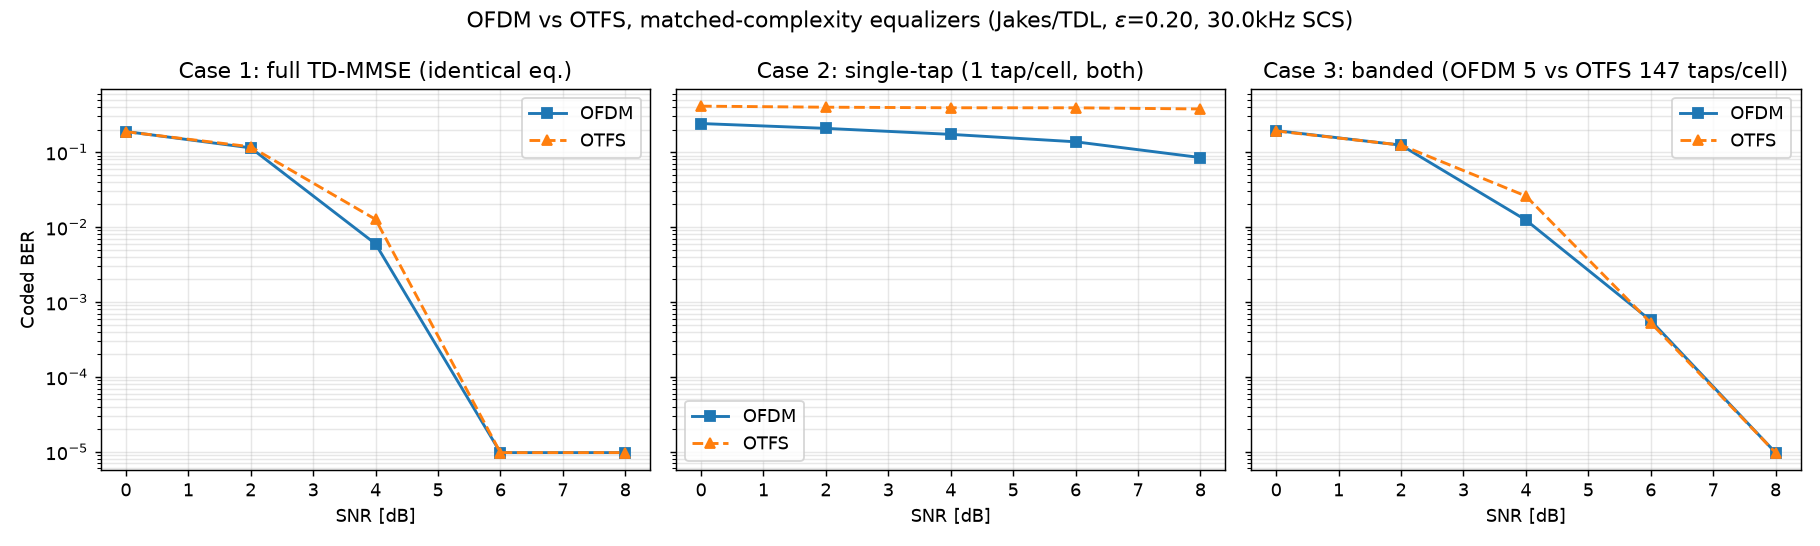
\includegraphics[width=\linewidth]{cases_jakes.png}
\caption{Matched-complexity OFDM vs.\ OTFS on a Jakes/TDL channel with fractional
delays ($\varepsilon{=}0.2$, $30$\,kHz SCS, LDPC). Case 1: the same full
equalizer makes them equivalent. Case 2: single-tap OFDM far exceeds single-tap
OTFS (the FFT diagonalizes delay). Case 3: both floor under finite-band
equalization, OTFS lower but with $\sim\!30\times$ more taps.}
\label{fig:cases}
\end{figure}

\section{Numerical Illustration}
\label{sec:num}
We simulate a realistic doubly dispersive channel, a 3GPP-TDL-C-like profile with
fractional delays of $0$, $200$, $800$, and $1600$\,ns, a classical (Jakes)
Doppler spectrum, and eleven resolvable taps, at $M{=}64$ and $N{=}8$, QPSK, a
rate-$1/2$ length-$1024$
LDPC code with sum-product decoding, and a common frame interleaver applied
identically to all waveforms. We compare four receivers: standard CP-OFDM with
single-tap frequency-domain equalization, the proposed ZP-OFDM with the block
ICI-aware banded equalizer, FDE-OTFS (the OTFS spreading equalized by that same
per-symbol band), and OTFS with a joint banded delay--Doppler LMMSE.
Soft decoding uses bias-corrected MMSE demapping, in which each equalizer output
is de-biased and weighted by its own post-equalization SINR.
Fig.~\ref{fig:ber}(a) and (b) show mild ($\varepsilon_{\max}{=}0.3$) and severe
($\varepsilon_{\max}{=}1.2$) Doppler, corresponding at $3.5$\,GHz to about
$2800$ and $11000$\,km/h, the latter a deliberately extreme (LEO-like) stress
point. The CSI is perfect unless stated otherwise.

Four observations hold in both regimes. First, standard single-tap CP-OFDM lags
by several decibels and, under severe Doppler, floors above $10^{-1}$: the single
tap captures only the average subcarrier gain, and the code cannot repair the
systematic ICI left behind. Second, the proposed block ICI-aware ZP-OFDM removes
the floor entirely and waterfalls together with the delay--Doppler receiver.
Third, it tracks OTFS to within about $1$\,dB, measured as the horizontal gap at a
fixed coded BER, at both mild and severe Doppler, sitting a visible but small step
behind. The residual is a coding-gain effect rather than a diversity-order loss
(Sec.~\ref{sec:vs}): the equalizer removes the floor and the code recovers the
diversity. Fourth, FDE-OTFS, which applies the OTFS spreading but equalizes it
with the same per-symbol frequency-domain band as the proposed receiver,
coincides with ZP-OFDM rather than with the joint OTFS detector. The spreading
therefore confers no advantage once the equalizer is the cheap per-symbol one,
which is the empirical form of Remark~\ref{rmk:matched}: the delay--Doppler edge
comes from the joint equalizer, not from the modulation. The comparison is read in
the operating waterfall region, at coded BER between $10^{-2}$ and $10^{-4}$.
Below it both waveforms are noise-limited and coincide, and above it the
finite-band OFDM residual of Sec.~\ref{sec:vs} appears, pushed down by a wider
Doppler-matched band. The gap is robust to the frame shape. Doubling the Doppler
dimension to $N{=}16$, which gives OTFS more delay--Doppler diversity to harvest,
still leaves the adaptive OFDM within about $1$\,dB of the OTFS genie.

Under imperfect CSI, both waveforms estimate the time-varying taps from
equivalent time-domain pilots, since the OTFS delay--Doppler pilot is a
Doppler-precoded time-domain pilot. A 20\,dB pilot shifts both curves right by
about 2 to 3\,dB while preserving their ordering, and banding regularizes the
estimation error in both domains. The degradation is thus comparable, since both
receivers estimate the same channel from pilots of the same quality.

\begin{figure}[!t]
\centering
\begin{subfigure}{0.49\linewidth}
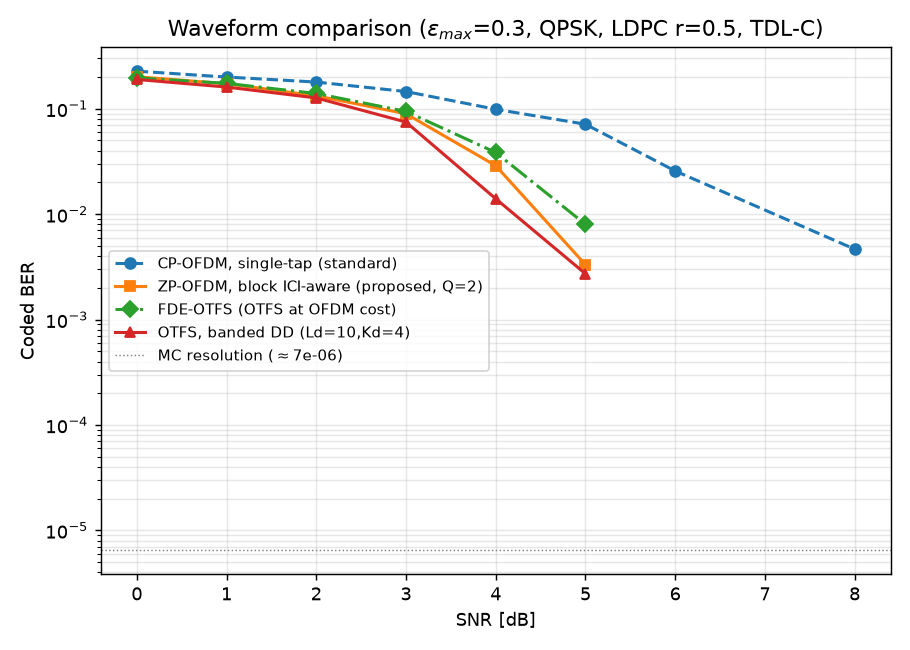
\includegraphics[width=\linewidth]{ber_eps03.png}
\caption{Mild Doppler, $\varepsilon_{\max}{=}0.3$.}
\label{fig:eps03}
\end{subfigure}
\hfill
\begin{subfigure}{0.49\linewidth}
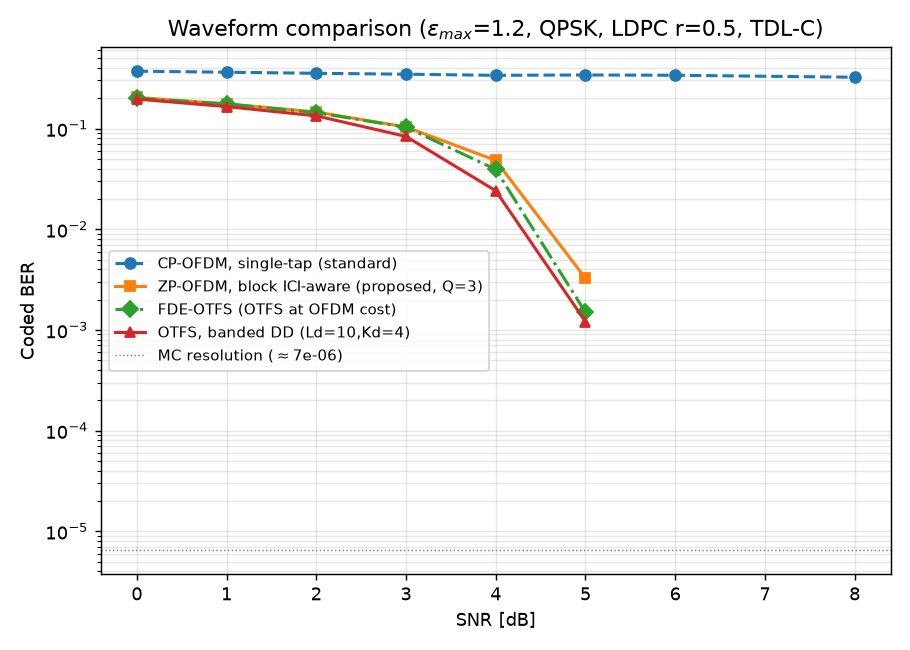
\includegraphics[width=\linewidth]{ber_eps12.png}
\caption{Severe Doppler, $\varepsilon_{\max}{=}1.2$ (LEO-like).}
\label{fig:eps12}
\end{subfigure}
\caption{Coded BER of four receivers on a realistic 3GPP-TDL-C channel (fractional
delays, Jakes Doppler, eleven taps), LDPC, $M{=}64$, $N{=}8$. Standard single-tap
CP-OFDM lags at mild Doppler and floors above $10^{-1}$ at severe Doppler. The
proposed block ICI-aware ZP-OFDM removes the floor and comes within about $1$\,dB
of the joint banded delay--Doppler OTFS. FDE-OTFS, the OTFS spreading equalized at
OFDM complexity, coincides with the proposed ZP-OFDM rather than with joint OTFS,
so the spreading gives no gain without the costlier joint equalizer
(Remark~\ref{rmk:matched}). The dotted line marks the Monte-Carlo resolution.}
\label{fig:ber}
\end{figure}

\section{Pulse Shaping and Spectral Containment}
\label{sec:pulse}
Practical deployments must meet a spectral mask, which rectangular-pulse OFDM
(and, more so, rectangular-pulse OTFS) violates through slowly decaying sidelobes.
A transmit filter (filtered-OFDM) restores containment, and it composes cleanly
with the ICI-aware equalizer. A filter is linear and time-invariant, so when its
memory fits within the CP/ZP guard the guard turns it into a circular convolution
that the DFT diagonalizes. It then appears as a per-subcarrier gain $G_k$ rather
than as inter-carrier leakage. Orthogonality is thus preserved, and the only cost
is attenuation of the edge subcarriers in the transition band, which are made
null guards. Should the filter exceed the guard for a sharper roll-off, the small
residual ICI it creates is exactly of the banded form that the multitap equalizer
already removes.

Fig.~\ref{fig:pulse} confirms this for a $64$-point FFT with $48$ data and $16$
null subcarriers, QPSK, LDPC coding, and the ICI-aware equalizer ($Q{=}2$). The
filtered spectrum meets a $-40$\,dB mask that rectangular OFDM and OTFS both
violate, while the coded BER tracks the rectangular case within about 1\,dB, the
edge-subcarrier margin, and reaches the same floor. Pulse shaping and adaptive ICI-aware
equalization are therefore compatible. The delay--Doppler domain, by contrast,
requires its own realizable pulse such as ODDM to achieve comparable containment.

\begin{figure}[!ht]
\centering
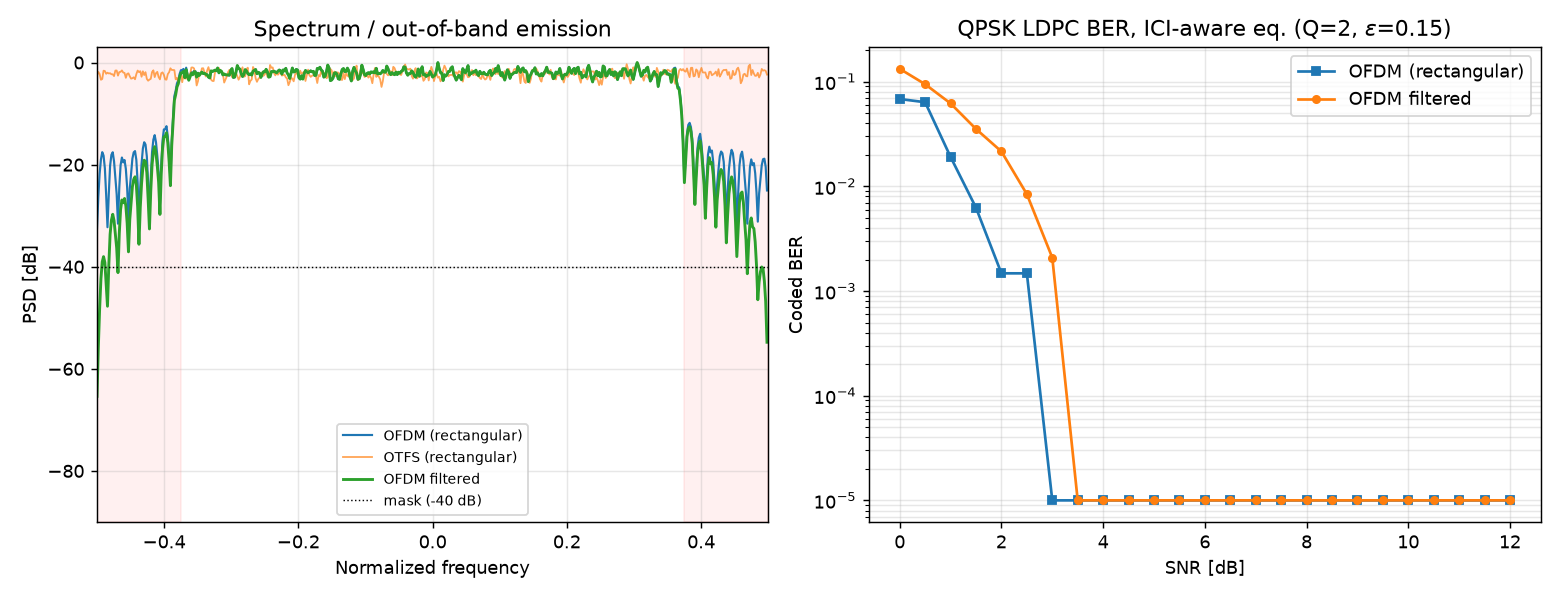
\includegraphics[width=0.92\linewidth]{pulse_shaping.png}
\caption{Pulse shaping. Left: a transmit filter (filtered OFDM) meets a
$-40$\,dB spectral mask that rectangular OFDM and rectangular OTFS violate.
Right: LDPC-coded QPSK BER with the ICI-aware equalizer. Filtered OFDM tracks the
rectangular case within about 1\,dB, the edge-subcarrier margin.}
\label{fig:pulse}
\end{figure}

\section{Conclusion}
Sizing an OFDM ICI equalizer from the delay--Doppler channel estimate adapts the
band to the ICI level, and thereby the order to the mobility. This removes the
doubly-dispersive error floor at a cost that scales with the Doppler spread
rather than the frame size. Under identical coding and interleaving the receiver
comes within about $1$\,dB of a delay--Doppler OTFS detector, at both mild and
severe Doppler, while remaining per-symbol, parallel, and roughly two
orders of magnitude cheaper in equalization. The comparison exposes a clean
division of labour. The diversity of the doubly dispersive channel is harvested
either in the equalizer, as OTFS does with a complex joint delay--Doppler
detector, or in the code and interleaver, as OFDM does. Since the two attain the
same diversity order, the choice is where to spend complexity, and OFDM pays for
it with a strong code, deep interleaving, and a Doppler-matched band. A symbol
spreading precode such as FTI-OFDM~\cite{Stolfi2006} is a further option that
adds this diversity in the modulation, at OFDM equalizer cost. It is worth noting
that integrated sensing and communication is not exclusive to OTFS in this
setting, since the time-domain pilots produce a delay--Doppler image of the
channel that the proposed receiver can directly reuse for sensing. What the
delay--Doppler domain may still offer beyond this recoverable diversity is the
model-free channel predictability of Zak-OTFS, which is its more durable
justification. Reaching the last fraction of a decibel, a band-limited pilot for
spectrally constrained deployments, and a full-scale (5G-sized) BER validation
are left as future work.

\begin{thebibliography}{99}
\bibitem{Muquet2002} B.~Muquet \emph{et al.}, ``Cyclic prefixing or zero padding
for wireless multicarrier transmissions?,'' \emph{IEEE Trans.\ Commun.},
vol.~50, no.~12, pp.~2136--2148, 2002.
\bibitem{Jeon1999} W.~G.~Jeon, K.~H.~Chang, and Y.~S.~Cho, ``An equalization
technique for OFDM systems in time-variant multipath channels,'' \emph{IEEE
Trans.\ Commun.}, vol.~47, no.~1, pp.~27--32, 1999.
\bibitem{Cai2003} X.~Cai and G.~B.~Giannakis, ``Bounding performance and
suppressing intercarrier interference in wireless mobile OFDM,'' \emph{IEEE
Trans.\ Commun.}, vol.~51, no.~12, pp.~2047--2056, 2003.
\bibitem{Rugini2005} L.~Rugini, P.~Banelli, and G.~Leus, ``Simple equalization
of time-varying channels for OFDM,'' \emph{IEEE Commun.\ Lett.}, vol.~9, no.~7,
pp.~619--621, 2005.
\bibitem{Rugini2006} L.~Rugini, P.~Banelli, and G.~Leus, ``Low-complexity banded
equalizers for OFDM systems in Doppler spread channels,'' \emph{EURASIP J.\ Adv.\
Signal Process.}, Art.\ 67404, 2006.
\bibitem{Raviteja2019} P.~Raviteja, Y.~Hong, and E.~Viterbo, ``Embedded
pilot-aided channel estimation for OTFS in delay--Doppler channels,'' \emph{IEEE
Trans.\ Veh.\ Technol.}, vol.~68, no.~5, pp.~4906--4917, 2019.
\bibitem{Stolfi2006} G.~Stolfi and L.~A.~Baccal\'a, ``Fourier transform time
interleaving in OFDM modulation,'' in \emph{Proc.\ IEEE Int.\ Symp.\ Spread
Spectrum Techn.\ Appl.\ (ISSSTA)}, 2006, pp.~322--326.
\bibitem{Muck2006} M.~Muck, M.~de Courville, and P.~Duhamel, ``A pseudorandom
postfix OFDM modulator---semi-blind channel estimation and equalization,''
\emph{IEEE Trans.\ Signal Process.}, vol.~54, no.~3, pp.~1005--1017, 2006.
\end{thebibliography}

\end{document}
